\documentclass[a4paper,12pt,twoside]{memoir}

% Castellano
\usepackage[spanish,es-tabla]{babel}
\selectlanguage{spanish}
\usepackage[utf8]{inputenc}
\usepackage[T1]{fontenc}
\usepackage{lmodern} % scalable font
\usepackage{microtype}
\usepackage{placeins}
\usepackage{eurosym}
\usepackage{pdflscape}
\usepackage{listings}

\RequirePackage{booktabs}
\RequirePackage[table]{xcolor}
\RequirePackage{xtab}
\RequirePackage{multirow}

% Links
\PassOptionsToPackage{hyphens}{url}\usepackage[colorlinks]{hyperref}
\hypersetup{
	allcolors = {red}
}

% Ecuaciones
\usepackage{amsmath}

% Rutas de fichero / paquete
\newcommand{\ruta}[1]{{\sffamily #1}}

% Párrafos
\nonzeroparskip

% Huérfanas y viudas
\widowpenalty100000
\clubpenalty100000

% Evitar solapes en el header
\nouppercaseheads

% Imagenes
\usepackage{graphicx}
\newcommand{\imagen}[2]{
	\begin{figure}[!h]
		\centering
		\includegraphics[width=0.9\textwidth]{#1}
		\caption{#2}\label{fig:#1}
	\end{figure}
	\FloatBarrier
}

\newcommand{\imagenflotante}[2]{
	\begin{figure}%[!h]
		\centering
		\includegraphics[width=0.9\textwidth]{#1}
		\caption{#2}\label{fig:#1}
	\end{figure}
}



% El comando \figura nos permite insertar figuras comodamente, y utilizando
% siempre el mismo formato. Los parametros son:
% 1 -> Porcentaje del ancho de página que ocupará la figura (de 0 a 1)
% 2 --> Fichero de la imagen
% 3 --> Texto a pie de imagen
% 4 --> Etiqueta (label) para referencias
% 5 --> Opciones que queramos pasarle al \includegraphics
% 6 --> Opciones de posicionamiento a pasarle a \begin{figure}
\newcommand{\figuraConPosicion}[6]{%
  \setlength{\anchoFloat}{#1\textwidth}%
  \addtolength{\anchoFloat}{-4\fboxsep}%
  \setlength{\anchoFigura}{\anchoFloat}%
  \begin{figure}[#6]
    \begin{center}%
      \Ovalbox{%
        \begin{minipage}{\anchoFloat}%
          \begin{center}%
            \includegraphics[width=\anchoFigura,#5]{#2}%
            \caption{#3}%
            \label{#4}%
          \end{center}%
        \end{minipage}
      }%
    \end{center}%
  \end{figure}%
}

%
% Comando para incluir imágenes en formato apaisado (sin marco).
\newcommand{\figuraApaisadaSinMarco}[5]{%
  \begin{figure}%
    \begin{center}%
    \includegraphics[angle=90,height=#1\textheight,#5]{#2}%
    \caption{#3}%
    \label{#4}%
    \end{center}%
  \end{figure}%
}
% Para las tablas
\newcommand{\otoprule}{\midrule [\heavyrulewidth]}
%
% Nuevo comando para tablas pequeñas (menos de una página).
\newcommand{\tablaSmall}[5]{%
 \begin{table}
  \begin{center}
   \rowcolors {2}{gray!35}{}
   \begin{tabular}{#2}
    \toprule
    #4
    \otoprule
    #5
    \bottomrule
   \end{tabular}
   \caption{#1}
   \label{tabla:#3}
  \end{center}
 \end{table}
}

%
%Para el float H de tablaSmallSinColores
\usepackage{float}

%
% Nuevo comando para tablas pequeñas (menos de una página).
\newcommand{\tablaSmallSinColores}[5]{%
 \begin{table}[H]
  \begin{center}
   \begin{tabular}{#2}
    \toprule
    #4
    \otoprule
    #5
    \bottomrule
   \end{tabular}
   \caption{#1}
   \label{tabla:#3}
  \end{center}
 \end{table}
}

\newcommand{\tablaApaisadaSmall}[5]{%
\begin{landscape}
  \begin{table}
   \begin{center}
    \rowcolors {2}{gray!35}{}
    \begin{tabular}{#2}
     \toprule
     #4
     \otoprule
     #5
     \bottomrule
    \end{tabular}
    \caption{#1}
    \label{tabla:#3}
   \end{center}
  \end{table}
\end{landscape}
}

%
% Nuevo comando para tablas grandes con cabecera y filas alternas coloreadas en gris.
\newcommand{\tabla}[6]{%
  \begin{center}
    \tablefirsthead{
      \toprule
      #5
      \otoprule
    }
    \tablehead{
      \multicolumn{#3}{l}{\small\textsl continúa desde la página anterior}\\
      \toprule
      #5
      \otoprule
    }
    \tabletail{
      \hline
      \multicolumn{#3}{r}{\small\textsl continúa en la página siguiente}\\
    }
    \tablelasttail{
      \hline
    }
    \bottomcaption{#1}
    \rowcolors {2}{gray!35}{}
    \begin{xtabular}{#2}
      #6
      \bottomrule
    \end{xtabular}
    \label{tabla:#4}
  \end{center}
}

%
% Nuevo comando para tablas grandes con cabecera.
\newcommand{\tablaSinColores}[6]{%
  \begin{center}
    \tablefirsthead{
      \toprule
      #5
      \otoprule
    }
    \tablehead{
      \multicolumn{#3}{l}{\small\sl continúa desde la página anterior}\\
      \toprule
      #5
      \otoprule
    }
    \tabletail{
      \hline
      \multicolumn{#3}{r}{\small\sl continúa en la página siguiente}\\
    }
    \tablelasttail{
      \hline
    }
    \bottomcaption{#1}
    \begin{xtabular}{#2}
      #6
      \bottomrule
    \end{xtabular}
    \label{tabla:#4}
  \end{center}
}

%
% Nuevo comando para tablas grandes sin cabecera.
\newcommand{\tablaSinCabecera}[5]{%
  \begin{center}
    \tablefirsthead{
      \toprule
    }
    \tablehead{
      \multicolumn{#3}{l}{\small\sl continúa desde la página anterior}\\
      \hline
    }
    \tabletail{
      \hline
      \multicolumn{#3}{r}{\small\sl continúa en la página siguiente}\\
    }
    \tablelasttail{
      \hline
    }
    \bottomcaption{#1}
  \begin{xtabular}{#2}
    #5
   \bottomrule
  \end{xtabular}
  \label{tabla:#4}
  \end{center}
}



\definecolor{cgoLight}{HTML}{EEEEEE}
\definecolor{cgoExtralight}{HTML}{FFFFFF}

%
% Nuevo comando para tablas grandes sin cabecera.
\newcommand{\tablaSinCabeceraConBandas}[5]{%
  \begin{center}
    \tablefirsthead{
      \toprule
    }
    \tablehead{
      \multicolumn{#3}{l}{\small\sl continúa desde la página anterior}\\
      \hline
    }
    \tabletail{
      \hline
      \multicolumn{#3}{r}{\small\sl continúa en la página siguiente}\\
    }
    \tablelasttail{
      \hline
    }
    \bottomcaption{#1}
    \rowcolors[]{1}{cgoExtralight}{cgoLight}

  \begin{xtabular}{#2}
    #5
   \bottomrule
  \end{xtabular}
  \label{tabla:#4}
  \end{center}
}




\graphicspath{ {./img/} }

% Capítulos
\chapterstyle{bianchi}
\newcommand{\capitulo}[2]{
	\setcounter{chapter}{#1}
	\setcounter{section}{0}
	\setcounter{figure}{0}
	\setcounter{table}{0}
	\chapter*{#2}
	\addcontentsline{toc}{chapter}{#2}
	\markboth{#2}{#2}
}

% Apéndices
\renewcommand{\appendixname}{Apéndice}
\renewcommand*\cftappendixname{\appendixname}

\newcommand{\apendice}[1]{
	%\renewcommand{\thechapter}{A}
	\chapter{#1}
}

\renewcommand*\cftappendixname{\appendixname\ }

% Formato de portada
\makeatletter
\usepackage{xcolor}
\newcommand{\tutor}[1]{\def\@tutor{#1}}
\newcommand{\course}[1]{\def\@course{#1}}
\definecolor{cpardoBox}{HTML}{E6E6FF}
\def\maketitle{
  \null
  \thispagestyle{empty}
  % Cabecera ----------------
\noindent
\includegraphics[width=\textwidth]{cabecera}\vspace{1cm}%
  \vfill
  % Título proyecto y escudo informática ----------------
  \colorbox{cpardoBox}{%
    \begin{minipage}{.8\textwidth}
      \vspace{.5cm}\Large
      \begin{center}
      \textbf{TFG del Grado en Ingeniería Informática}\vspace{.6cm}\\
      \textbf{\LARGE\@title{}}
      \end{center}
      \vspace{.2cm}
    \end{minipage}

  }%
  \hfill\begin{minipage}{.20\textwidth}
    
\includegraphics[width=\textwidth]{escudoInfor}
  \end{minipage}
  \vfill
  % Datos de alumno, curso y tutores ------------------
  \begin{center}%
  {%
    \noindent\LARGE
    Presentado por \@author{}\\ 
    en Universidad de Burgos --- \@date{}\\
    Tutor: \@tutor{}\\
  }%
  \end{center}%
  \null
  \cleardoublepage
  }
\makeatother


% Datos de portada
\title{Aplicación Android para la detección de retinopatía diabética}
\author{Miguel Fuente García}
\tutor{D. Daniel Urda Muñoz y D. Nuño Basurto Hornillos}
\date{\today}

\begin{document}

\maketitle



\cleardoublepage



%%%%%%%%%%%%%%%%%%%%%%%%%%%%%%%%%%%%%%%%%%%%%%%%%%%%%%%%%%%%%%%%%%%%%%%%%%%%%%%%%%%%%%%%



\frontmatter


\clearpage

% Indices
\tableofcontents

\clearpage

\listoffigures

\clearpage

\listoftables

\clearpage

\mainmatter

\appendix

\apendice{Plan de Proyecto Software}

\section{Introducción}

\section{Planificación temporal}
Para la planificación temporal, cabe destacar que se ha seguido la metodología SCRUM, la cual no se ha podido seguir al 100\%, puesto que es una metodología planeada para equipos de trabajo, siendo este un proyecto personal de final de carrera. 

\begin{itemize}
    \item se programó el \textit{sprint} de dos semanas, donde, se podrían haber hecho de una semana, pero la metodología SCRUM recomienda de dos a cuatro.
    \item Durante, el  \textit{sprint} se planean unas tareas a terminar en el periodo de tiempo.
    \item Cada tarea tiene un objetivo y una estimación; se organizan en un tablero canvas con las siguientes columnas consideradas:
    \begin{itemize}
        \item "tareas a realizar" : Son las tareas planeadas para el sprint actual o próximos.
        \item "tareas en proceso" : Son aquellas tareas que se están realizando en el momento.
        \item "tareas terminadas" : Son las tareas que ya se han terminado, las cuales se comprueban al final del sprint si se han terminado correctamente, en tal caso se cierran.
        \item "tareas cerradas" : Son aquellas tareas que se han cerrado en \textit{sprints} anteriores, las cuales se han implementado correctamente en el producto final. 
    \end{itemize}
    \item Con los gráficos \textit{burndown}, se puede observar el proceso del proyecto de cada \textit{sprint}
    \item Como se ha comentado, al terminar el sprint,se realizaba una reunión personal, donde se comprobaba si se habían completado correctamente las tareas terminadas. En caso de no ser así, se añadía para el siguiente \textit{sprint}, además, se añadían las nuevas tareas a realizar en el siguiente.
\end{itemize}
Esta metodología se ha implementado usando la herramienta ZenHub, la cual permite hacer los apartados anteriores con facilidad.
Para asignar los pesos de la tarea, se utiliza una aproximación de la secuencia de fibonacci. Donde los valores dependen del tiempo y dificultad que llevará la tarea, esta estimación, a lo largo del proyecto va siendo más precisa, puesto que al principio, no se controlaban los tiempos que conllevarían las dificultades del proyecto.

Los \textit{sprints} que se realizaron se comentan a continuación.

\subsection{Sprint 0 - Anterior al 27/12/2022}
En este sprint inicial, del que no se poseen fechas, se realizaron diversas reuniones, en las cuales se explicaron en que iba a consistir el proyecto.

Durante este sprint, se estuvo investigando sobre aplicaciones Android con el mismo objetivo, sobre las que basar el proyecto. Encontrando de esta forma la aplicación Ret-iN CaM. La cual sirve para realizar estudios sobre los pacientes, de forma que se pueda ver la evolución.
Además, se realizaron búsquedas sobre redes neuronales ya creadas las cuales añadir a la aplicación. 

Como este sprint fue más un periodo de búsqueda de información, sin realizar ningún trabajo real, no se contabilizó el trabajo realizado.
\subsection{Sprint 1 - 27/12/2022 - 10/01/2023}
En este primer Sprint, se estuvo pensando con que herramienta realizar el proyecto. Teniendo como objetivo crear tanto el proyecto, como el LaTeX.

Para la aplicación móvil, se pensaba utilizar o Android Studio o Unity, de Android Studio ya se tenían conocimientos de uso, pero de Unity no, por ello, se realizo un proyecto ''Hola Mundo'' en Unity, para ver la complejidad; al ver que la herramienta estaba más destinada a aplicaciones gráficas, se decidió realizar la aplicación en Android Studio, creando el proyecto.

Para la realización del documento, se pensó hacer de forma local, utilizando MiKTeX, pero por facilidad de uso de los tutores, quienes preferían el uso de OverLeaf, que les permitía corregir de forma concurrente el documento, se utilizó esta.

Como este primer sprint se estaba empezando, y además era Navidad, se olvidó mover las tareas de ZenHub a terminadas, y la gráfica que proporciona ZenHub es incorrecta. 

\imagen{burndown/primerSprint.png}{Sprint 1.}
\subsection{Sprint 2 - 10/01/2023 - 24/01/2023}
En el segundo Sprint se planeo hacer el menú principal de la aplicación, para ir haciendo la interfaz de usuario y a su vez, se hizo una investigación sobre que colores relaciona el ser humano con la retinopatía diabética.
Para hacer el menú, primero se hizo un boceto a mano, por ese motivo, se puso un valor alto de la estimación.
Por otro lado, se investigó sobre como implementar las redes neuronales en Android Studio, e ir añadiendo apartados al documento LaTeX.

De estas tareas, no se pudieron terminar ni la de investigar como implementar una red neuronal en Android Studio, ni añadir el apartado en concreto del LaTeX. Aunque si que se avanzó, SCRUM no permite dividir la tarea en parte terminada y parte que no, por lo que se va a considerar que no se han realizado.

El gráfico burndown se vería incorrectamente, debido al inconveniente ocurrido en el primer sprint, arreglando este defecto, se vería de esta forma:
\imagen{burndown/segundoSprint.png}{Sprint 2.}

\subsection{Sprint 3 - 24/01/2023 - 07/02/2023}
En el tercer Sprint, se añadieron las tareas no terminadas en el anterior, y se añadió también, el terminar el boceto inicial de la aplicación.
Al iniciar el sprint, se pensó en que la aplicación tenia que tener nombre y un logo, pero se programó para futuros sprints porque ya se tenían varias tareas para este.
Además, no se pudo avanzar mucho en la introducción del LaTeX porque era necesario aclarar una duda presencialmente, y la reunión se hizo a finales del sprint.

Como se iba avanzando en las tareas simultáneamente, tanto terminar el boceto de la aplicación y buscar información de la implementación, se terminaron el mismo día.
\imagen{burndown/tercerSprint.png}{Sprint 3.}
\subsection{Sprint 4 - 07/02/2023 - 21/02/2023}
Para el cuarto sprint, se planeó realizar como una investigación sobre como se podría incluir la aplicación en la play store, y sobre como integrar tensorflow en Android Studio.

Al investigar sobre la play store, se dio cuenta que era necesario realizar un pago de 25\$, por ese mismo motivo, se preguntó a los tutores, quienes dijeron que no hacia falta subir la aplicación a ninguna tienda.

Por otro lado, se terminaron las demás tareas, cumpliendo los objetivos del sprint. Y aunque se podría haber eliminado la tarea de investigación de la play store, el tiempo gastado en la investigación se había realizado, por lo que no se elimino.

El burndown queda de la siguiente manera:
\imagen{burndown/cuartoSprint.png}{Sprint 4.}

\subsection{Sprint 5 - 21/02/2023 - 07/03/2023}
Para este sprint, como no había tareas atrasadas, se añadieron la creación del logo y el nombre de la aplicación, de la investigación anterior de como implementar una red neuronal en Android Studio, el caso concreto de una red neuronal .h5; realizar cambios en la interfaz para añadir y quitar funcionalidad. Y añadir una base de datos; para lo que se pensó realizar un conjunto de clases java, las cuales simulaban la base de datos, y con un constructor, inicializar los datos.

Debido a que no se me da muy bien en el diseño artístico, se me ocurrió la idea de utilizar la herramienta DALL·E2 para un diseño preliminar, una vez se proporcionó un resultado aceptable, se editó el icono eliminando ruido, y cambiando los colores.

Debido a las diversas actividades designadas en este sprint, no se pudo realizar la base de datos.
\imagen{burndown/quintoSprint.png}{Sprint 5.}

\subsection{Sprint 6 - 07/03/2023 - 21/03/2023}
En el sexto sprint, se añadieron realizar el apartado de trabajos relacionados del documento LaTeX, y probar una integración de una red neuronal básica.
Ambas tareas se terminaron, y se avanzo en la creación de la base de datos; pero no se terminó debido a que se querían añadir más datos, los cuales solo se crearon un médico, un paciente y un informe.

Sin contar que se podría haber considerado como la tarea terminada, el gráfico burndown, seria este:
\imagen{burndown/sextoSprint.png}{Sprint 6.}

\subsection{Sprint 7 - 21/03/2023 - 04/04/2023}
En este sprint, se termino la base de datos añadiendo otro par de pacientes y médicos, y se planearon hacer una eliminación de bugs, debido al modo oscuro, y que no guardaba bien datos entre las distintas actividades. Y también se pensó hacer el apartado "añadir técnicas y herramientas", pero se avanzó, sin poder acabar la tarea. Quedando para la siguiente actividad.

\imagen{burndown/septimoSprint.png}{Sprint 7.}



\section{Estudio de viabilidad}
Este proyecto, al estar orientado a la sanidad publica, no busca obtener beneficios, sino a facilitar la labor del médico.

En caso de querer desarrollar este proyecto con una intención comercial.

\subsection{Viabilidad económica}
\textbf{Costes}

\textbf{En personal}

Para el desarrollo del proyecto, se ha habría contratado a un programador \textit{junior} a tiempo parcial durante siete meses. 
Para la cotización de la seguridad social, se consideran los siguientes porcentajes:  un 23,60\% debido a las contingencias comunes, debido al desempleo de tipo general, al ser un contrato de tiempo indefinido, es un 5,50\%; un 0,2\% para el Fondo de Garantía Salarial, y un 0,60\% para formación profesional. Sumando estos porcentajes, un 29,9\% de retribución a la seguridad social.

\tablaSmall{Costes de personal}{l  c} {costesDePersonal}{Concepto & Coste\\} 
    {			Salario mensual neto & $973 $\euro\\
                Tipo de retención del IRPF & $11.69\%$\\
			Cuota a pagar del IRPF  & $195 $\euro\\
			Seguridad Social (29.9\%)& $498 $\euro\\
			Salario mensual bruto & $1.666 $\euro\\
			\hline
			\textbf{Total 6 meses} & $9.996 $\euro\\}

El coste se puede ver en la tabla: \ref{tabla:costesDePersonal}

\textbf{En \textit{hardware}}

Para realizar el proyecto, se hará uso de un ordenador portátil y opcionalmente, un dispositivo móvil, para comprobar el correcto funcionamiento de la aplicación.

Suponiendo que los dispositivos hardware se amortizan en seis años, y se han utilizado durante siete meses:

\tablaSmall{Costes de Hardware}{l  cc} {costesDeHardware}{Concepto & Coste & Amortización\\} 
    {			Ordenador & $1.200 $\euro & $100 $\euro\\
                Dispositivo móvil & $300 $ \euro & $25 $ \euro\\
                Oftalmoscopio Portátil D-Eye & $400 $\euro & $33,33 $\euro \\
			\hline
			\textbf{Total} & $1.900 $\euro & $158,33$\euro\\}

El coste se puede ver en la tabla: \ref{tabla:costesDeHardware}

\textbf{En \textit{software}}

Se muestran aquellas licencias de \textit{software} que no son gratuitas, y considerando que su amortización es de un año.
\tablaSmall{Costes de Software}{l  cc} {costesDeSoftware}{Concepto & Coste & Amortización\\} 
    {			Windows 11 Pro & $259 $\euro & $129,5 $\euro\\
                ZenHub para equipos (3 meses) & $36 $\euro & $18 $\euro\\
			\hline
			\textbf{Total} & $295 $\euro & $147,5 $\euro\\}

El coste se puede ver en la tabla: \ref{tabla:costesDeSoftware}
   
\textbf{Costes adicionales}

Como se pretende comercializar la aplicación, la \textit{Play Store} es una de las mejores plataformas de distribución de aplicaciones móviles. Pero, para publicar una aplicación, es necesario una cuenta de desarrollador, la cual cuesta 25€.
\tablaSmall{Costes adicionales}{l  c} {costesAdicionales}{Concepto & Coste\\} 
    {			Cuenta de desarrollador Play Store & $25 $\euro\\
                Internet & $210 $\euro \\
                Alquiler de oficina & $800 $\euro \\
			\hline
			\textbf{Total} & $1.035 $\euro \\}

   El coste se puede ver en la tabla: \ref{tabla:costesAdicionales}

\textbf{Costes totales}

Siendo los costes totales, los vistos en: \ref{tabla:costesAdicionales}
\tablaSmall{Costes totales}{l  c} {costesTotales}{Concepto & Coste\\} 
    {			En personal & $9.996 $\euro\\
                En hardware & $1.900 $\euro \\
                En software & $295 $\euro \\
                Adicionales & $1.035 $\euro \\
			\hline
			\textbf{Total} & $13.226 $\euro \\}

\textbf{Beneficios}

Como se ha comentado anteriormente, el proyecto tiene un objetivo altruista de ayudar en la labor del médico, dejando a un lado el objetivo de lucrarse con el proyecto. Hay varios focos en los que se podrían obtener beneficios:
\begin{itemize}
    \item Vender la aplicación al servicio sanitario, con un beneficio del 30\%. Dando la opción de comprar servicios de mantenimiento.
    \item Ofrecer licencias de la aplicación, cobrando cada año por mantener la suscripción.
    \item Introducir un anuncios en la aplicación.
    \item Distintas licencias de la aplicación, cada una con unas ventajas, con diferentes precios.
\end{itemize}

Entre las opciones anteriores, se ha descartado el uso de anuncios, principalmente, porque elimina profesionalidad a la aplicación; y también la opción de las distintas licencias, pero al ofrecer un único servicio, no se podía plantear esta opción.

Como las otras dos opciones se han considerado viables, se desarrollaran a continuación, además, es importante recalcar que los valores pueden  cambiar debido a la gran cantidad de centro sanitarios públicos que hay, proporcionando ofertas según esa cantidad.

\textbf{Vender la aplicación}

Vendiendo la aplicación al servicio sanitario, solo se realizaría un pago por la compra, de forma que la empresa obtenga un 30\% de beneficios.
De esta forma, $13.226 $\euro seria el 70\% del precio y la aplicación se vendería por $18.894,28$\euro; dando un beneficio de $5.668,28 $\euro. 

También se podría ofrecer al servicio sanitario una opción de compra, donde la empresa se encarga de hacer el mantenimiento y actualizaciones de la aplicación. Siendo un servicio que depende del numero de centros sanitarios que haya en la comunidad autónoma. Un posible precio razonable, seria que por cada centro sanitario, anualmente se pague una tarifa de $10 $\euro. 

Poniendo el caso de que el SACYL comprase la aplicación para el 25\% de los centros sanitarios, como tiene 10.218,
debería pagar por $(10.218 · 0,25 · 10 ) $, siendo de esta forma anualmente se alcanzaría una cifra de $25.545 $\euro al año.
Como una persona cuesta cada 6 meses, $9.996 $\euro, al año serian $19.992 $\euro, teniendo beneficios anuales.


\textbf{Licencias de la aplicación}

Como el caso anterior, se va a hacer una oferta por cada centro sanitario, donde anualmente, se cobraría $100 $\euro.

Suponiendo que el SACYL pidiese una licencia para todos los centros, se haría el calculo de $(10.218 · 0,25 · 100 ) $ dando una cifra anual de $255.450 $\euro en este precio ya estaría incluido el precio del mantenimiento.

En este caso, la empresa se encargaría de ofrecer los servicios al SACYL, se debería contratar un servidor con una base de datos, como el servidor guarda imágenes, se necesitaría bastante espacio, pongamos que se contrata un servidor Microsoft SQL Server de 1 GB, con un precio de $350$\euro al mes. Como 1GB pueden ser poco para Castilla y León, se considera que se compran 50 servidores. Añadiendo al coste anual, $4200 · 50 $ siendo así, $210.000 $\euro

Por tanto, con $255.450 $\euro al año; habría que restar el coste de los servidores y el del personal donde se podría aumentar el número a 2 personas,   $255.450 - 210.000 - 39.984 $, haciendo que anualmente, se tengan $5.466 $\euro de beneficio, como el coste de la aplicación era de 
 $13.226 $\euro, harían falta 3 años para obtener un beneficio real sobre el proyecto.

\textbf{Otros casos}

Hay un caso que es importante destacar, y es el caso concreto de que el SACYL fuese la empresa encargada.

En este caso, no hay ningún beneficio monetario para la empresa, puesto que es sanidad publica. Pero, realizando el proyecto, a futuro se pueden evitar costes adicionales, como por ejemplo: 
\begin{itemize}
    \item Coste de transporte de la ambulancia.
    \item Costes de citas innecesarias y el tiempo que conllevan estas.
    \item Costes de material utilizado.
\end{itemize}

\subsection{Viabilidad legal}

\textbf{Software}

Esta sección aborda el contexto legal del proyecto, junto con las licencias \textit{software} utilizadas.
\tabla{Dependencias del proyecto Android}{|p{3cm}|c|p{5cm}|c|}{4}{dependenciasAndroid}{Dependencia & Versión & Descripción & Licencia\\}{
Appcompat & 1.6.1 & Permite a versiones anteriores de Android una compatibilidad mejorada & Apache License 2.0\\
Material  & 1.8.0 & Proporciona componentes de Material Design para Android. & Apache License 2.0\\
Constraint Layout & 2.1.4 & Permite crear diseños complejos y flexibles & Apache License 2.0 \\
JUnit & 4.13.2 & Framework de pruebas unitarias en Java & Eclipse Public License \\
Ext JUnit & 1.1.5 & Biblioteca de pruebas unitarias para Android que extiende JUnit & Apache License 2.0\\
Espresso-core & 3.5.1 & Biblioteca de pruebas de interfaz de usuario & Apache License 2.0 \\
TensorFlow Lite & 2.7.0 & Biblioteca de aprendizaje automático, más ligera que TensorFlow & Apache License 2.0 \\
SQLite & 2.2.0 & Biblioteca que utiliza bases de datos SQLite, proporcionando una API para interactuar con la base de datos & No requiere\\
}

Como el proyecto también ha tenido una parte realizada en python, se incluyen las dependencias utilizadas, donde solo se usa la biblioteca de tensorflow, ya comentada anteriormente.

\textbf{Imágenes}

Hay varios tipos de imágenes utilizadas en el proyecto, donde el logo, se ha utilizado usando DALLE2, la cual en sus políticas y términos se explica que el usuario tiene todos los derechos, tanto comerciales y no comerciales.

Por otro lado, para los iconos de la aplicación, se usaron tanto iconos por defecto de Android Studio, como iconos de Google Fonts, donde todas las imágenes son de código abierto y no tienen costo. Con una licencia Apache 2.0.

Y por ultimo, las imágenes de la retina, 


\textbf{Licencia del proyecto}



\subsection{Marco legal del proyecto}

Es importante recalcar que al estar trabajando sobre una aplicación que usa datos delicados de las personas, siendo estos, además, datos relacionados con la salud. 

\textbf{RGPD}

Según viene descrito en el articulo 9 del Reglamento General de Protección de Datos, esta prohibido hacer un tratamiento de categorías especiales de datos personales a menos que ocurra:
\begin{itemize}
    \item El interesado ha dado el consentimiento explicito para el tratamiento de datos.
    \item Resulte necesario para proteger los intereses vitales del interesado u otra persona física cuando no este capacitado para dar su consentimiento.
    \item Es necesario para fines de medicina preventiva o laboral.
    \item Es necesario con fines de archivo en interés público, fines de investigación científica o histórica o fines estadísticos.
\end{itemize}

En el \href{https://www.boe.es/doue/2016/119/L00001-00088.pdf#page=38}{articulo 9}, vienen más puntos, pero solo se explican los referentes al uso de la aplicación.

En el \href{https://www.boe.es/doue/2016/119/L00001-00088.pdf#page=47}{capitulo 4} del Reglamento General de Protección de Datos, se trata sobre el responsable de  tratar los datos y  el encargado del tratamiento.

Por ello, con el fin de evitar que los datos sensibles se confundan entre los distintos pacientes, se ha implementado una interfaz, en la cual el médico introduce el DNI del paciente a ser tratado en ese momento, mostrando el nombre del paciente del DNI, en caso de haberse confundido a la hora de poner el DNI, se podrá dar cuenta al ver el nombre del paciente. 

\apendice{Especificación de Requisitos}

\section{Introducción}

En este apartado, se recogen los requisitos del proyecto, ya sean requisitos funcionales o no funcionales.

Como el proyecto se pueden dividir en dos proyectos, la aplicación Android y la creación de una red neuronal convolucional, se separarán estos entre sí, para una mayor visibilidad.

\section{Objetivos generales}

Los objetivos del proyecto Android buscan:

\begin{itemize}
    \item Proporcionar a los centros sanitarios una aplicación, que permita diferenciar cuándo un paciente posee o no retinopatía diabética.
    \item Guardar las respectivas imágenes en los pacientes indicados, con el resultado proporcionado.
    \item Mostrar los resultados para que el médico pueda proporcionar un primer diagnóstico.
\end{itemize}

Los objetivos del proyecto de la red neuronal:

\begin{itemize}
    \item Desarrollar un modelo que diferencie entre fotos con calidad buena y fotos con calidad mala.
    \item Desarrollar un modelo que clasifique correctamente el mayor número de instancias.
\end{itemize}

\section{Catálogo de requisitos}

Los requisitos funcionales para la aplicación Android son:
\begin{itemize}
    \item \textbf{RF-1: Gestión de usuarios}: Se desea que la aplicación permita gestionar los usuarios.
        \begin{itemize}
            \item \textbf{RF-1.1: Gestión de médicos}
            \begin{itemize}
                \item \textbf{RF-1.1.1: Mostrar datos médico}: Se desea poder ver los datos de los médicos.
            \end{itemize}
            \item \textbf{RF-1.2: Gestión de pacientes}
            \begin{itemize}
                \item \textbf{RF-1.2.1: Mostrar datos paciente}: Se desea poder ver los datos de los pacientes.
                
            \end{itemize}
            \end{itemize}
 
    \item \textbf{RF-2: Gestión de informes}: Se desea que la aplicación permita gestionar los informes.
        \begin{itemize}
            \item \textbf{RF-2.1: Creación de informes}: Se desea que los médicos puedan crear un informe a partir de una foto y un paciente.
            \begin{itemize}
                \item \textbf{RF-2.1.1: Obtención de fecha}: La aplicación debe tomar la fecha en la que se crea el informe.
                \item \textbf{RF-2.1.2: Obtención del ojo}: La aplicación debe tomar el ojo al que se va a realizar la foto.
                \item \textbf{RF-2.1.3: Obtención de la imagen}: La aplicación debe mostrar la opción de cómo realizar la imagen.
                \begin{itemize}
                        \item \textbf{RF-2.1.3.1: Tomar fotos}: Se desea que la aplicación permita tomar fotos de la cámara del usuario.
                        \item \textbf{RF-2.1.3.2: Escoger fotos}: Se desea que la aplicación permita escoger una foto desde la galería del paciente.
                        \item \textbf{RF-2.1.3.3: Calidad de la foto}: Se desea implementar un sistema que permita comprobar que la foto tomada es de calidad. En caso contrario, mostrar al usuario que la imagen no tiene una calidad aceptable, y que tome otra foto.
                \end{itemize}
                \item \textbf{RF-2.1.4: Obtención del resultado}: Se desea que la aplicación de un resultado basado en una red neuronal.
                \begin{itemize}
                    \item \textbf{RF-2.1.4.1: Escoger red neuronal}: Se desea que el usuario pueda elegir con que red neuronal analizar la imagen con la que obtener los resultados.
                \end{itemize}
            \end{itemize}
            \item \textbf{RF-2.2: Mostrar informes}: Se desea poder ver los informes según el paciente.
        \end{itemize}
    \item \textbf{RF-3: Iniciar sesión}: Se desea que la aplicación permita iniciar sesión.  
    \begin{itemize}
        \item \textbf{RF-3.1: Iniciar sesión como médico}: Los médicos pueden iniciar sesión con su email y su contraseña.
        \item \textbf{RF-3.2: Iniciar sesión como invitado}: Los médicos pueden iniciar sesión sin proporcionar email ni contraseña.
    \end{itemize}
    \item \textbf{RF-4: Escoger un paciente}: Se desea que el médico identificado introduzca el DNI de un paciente para gestionar sus informes o datos.
\end{itemize}

Requisitos no funcionales:

\begin{itemize}

    \item \textbf{RFNF-1: Base de datos}: Se debe almacenar los datos introducidos.
    \begin{itemize}
        \item \textbf{RFNF-1.1: Datos de los médicos}: Se desea almacenar la contraseña y el centro médico donde trabaja el médico.
        \item \textbf{RFNF-1.2: Datos de los pacientes}: Se desea almacenar una lista de informes, información sobre el paciente y el estado en el que se encuentra.
        \item \textbf{RFNF-1.3: Datos de los usuarios}: Se desea almacenar nombre, apellidos, fecha de nacimiento, DNI y el correo electrónico de los usuarios.
        \item \textbf{RFNF-1.4: Datos de los informes}: Se desea almacenar la foto del informe, la fecha en la que se obtuvo, el ojo al que hace referencia y el resultado de dicho informe. 
    \end{itemize}
    \item \textbf{RFNF-2: Concurrencia}: El usuario debe poder utilizar la aplicación mientras se comprueban las imágenes.
    \item \textbf{RFNF-3: Aplicación}: La aplicación debe funcionar correctamente, no dando errores al usuario y en caso de algún error, controlarlo.
    \item \textbf{RFNF-4: Interfaz}: La interfaz debe ser sencilla, para que usuarios nuevos puedan utilizarla.
    \item \textbf{RFNF-5: Dispositivos}: La aplicación debe ejecutarse correctamente en el máximo número de dispositivos.
\end{itemize}

Por otro lado, no hay requisitos funcionales para el proyecto de la red neuronal, siendo los requisitos no funcionales:
\begin{itemize}
    \item \textbf{RFNF-1: Red neuronal de calidad}: Se debe crear una red neuronal que diferencie entre una calidad APTA y una calidad NO\_APTA.
    \item \textbf{RFNF-2: Escoger el mejor modelo}: Se debe escoger el mejor modelo obtenido.
\end{itemize}
\section{Actores}
Para la aplicación se consideran 2 actores, pero se podría considerar solo uno.
\begin{itemize}
    \item \textbf{Actor médico}: Este actor es un médico identificado, quien ha iniciado sesión con su email y contraseña; además, proporciona el DNI del paciente para trabajar sobre el paciente que ha ido a consulta.
    \item \textbf{Actor invitado}: Este actor es un médico no identificado, de esta forma, puede comprobar el grado de retinopatía diabética sin crear un informe a un paciente. Este actor es el indicado, cuando se ha proporcionado una imagen a analizar y no se sabe el paciente en concreto.
\end{itemize}


\section{Especificación de requisitos}

En este apartado se explicarán los casos de uso.


\begin{landscape}
\textbf{Diagrama de casos de uso}
\begin{figure}[!ht]
         \centering
         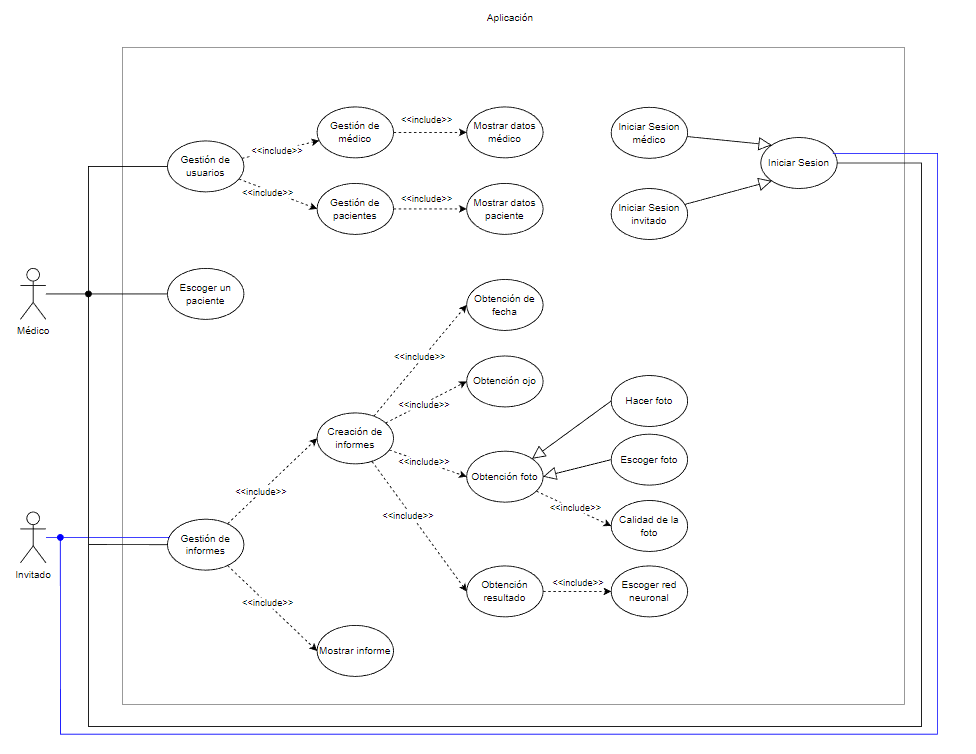
\includegraphics[height=0.8\textheight]{img/Diagrama de casos de uso.png}
         \caption{Diagrama de casos de uso}
         \label{fig:Diagrama de casos de uso}
\end{figure}
\end{landscape}

\textbf{Casos de uso}

\begin{table}[h]
	\centering
	\begin{tabularx}{\linewidth}{ p{0.21\columnwidth} p{0.71\columnwidth} }
		\toprule
		\textbf{CU-1}    & \textbf{Gestión de usuarios}\\
		\toprule
		\textbf{Versión}              & 1.0    \\
		\textbf{Autor}                & Miguel Fuente García \\
		\textbf{Requisitos asociados} & RF-1, RF-1.1, RF-1.1.1, RF-1.2, RF-1.2.1  \\
		\textbf{Descripción}          & Se desea que la aplicación permita gestionar los usuarios. \\
		\textbf{Precondición}         & El médico debe estar identificado, y haya puesto un DNI de paciente valido. \\
		\textbf{Acciones}             &
		\begin{enumerate}
			\def\labelenumi{\arabic{enumi}.}
			\tightlist
			\item El usuario llega a la página principal de la aplicación.
			\item Se ofrece la opción de ver los datos del médico.
                \item Se ofrece la opción de ver los datos del paciente.
		\end{enumerate}\\
		\textbf{Postcondición}        &  \\
		\textbf{Excepciones}          &  \\
		\textbf{Importancia}          & Media  \\
		\bottomrule
	\end{tabularx}
	\caption{CU-1 Gestión de usuarios.}
\end{table}

\begin{table}[h]
	\centering
	\begin{tabularx}{\linewidth}{ p{0.21\columnwidth} p{0.71\columnwidth} }
		\toprule
		\textbf{CU-2}    & \textbf{Gestión de médico}\\
		\toprule
		\textbf{Versión}              & 1.0    \\
		\textbf{Autor}                & Miguel Fuente García \\
		\textbf{Requisitos asociados} & RF-1.1, RF-1.1.1  \\
  
		\textbf{Descripción}          & Se desea que la aplicación permita gestionar los médicos. \\
		\textbf{Precondición}         & El médico debe estar identificado. \\
		\textbf{Acciones}             &
		\begin{enumerate}
			\def\labelenumi{\arabic{enumi}.}
			\tightlist
			\item El usuario selecciona el botón para ver sus datos.
		\end{enumerate}\\
		\textbf{Postcondición}        &  \\
		\textbf{Excepciones}          &  \\
		\textbf{Importancia}          & Baja  \\
		\bottomrule
	\end{tabularx}
	\caption{CU-2 Gestión de médico.}
\end{table}

\begin{table}[p]
	\centering
	\begin{tabularx}{\linewidth}{ p{0.21\columnwidth} p{0.71\columnwidth} }
		\toprule
		\textbf{CU-3}    & \textbf{Mostrar datos médico}\\
		\toprule
		\textbf{Versión}              & 1.0    \\
		\textbf{Autor}                & Miguel Fuente García \\
		\textbf{Requisitos asociados} & RF-1.1.1 \\
		\textbf{Descripción}          & Se desea poder ver los datos de los médicos. \\
		\textbf{Precondición}         & El médico debe estar identificado. \\
		\textbf{Acciones}             &
		\begin{enumerate}
			\def\labelenumi{\arabic{enumi}.}
			\tightlist
			\item La aplicación obtiene los datos del médico de la base de datos.
            \item La aplicación muestra los datos del médico en la interfaz.
		\end{enumerate}\\
		\textbf{Postcondición}        &  \\
		\textbf{Excepciones}          &  \\
		\textbf{Importancia}          & Baja  \\
		\bottomrule
	\end{tabularx}
	\caption{CU-3 Mostrar datos médico.}
\end{table}

\begin{table}[p]
	\centering
	\begin{tabularx}{\linewidth}{ p{0.21\columnwidth} p{0.71\columnwidth} }
		\toprule
		\textbf{CU-4}    & \textbf{Gestión de pacientes}\\
		\toprule
		\textbf{Versión}              & 1.0    \\
		\textbf{Autor}                & Miguel Fuente García \\
		\textbf{Requisitos asociados} & RF-1.2, RF-1.2.1  \\
  
		\textbf{Descripción}          & Se desea que la aplicación permita gestionar los pacientes. \\
		\textbf{Precondición}         & El médico debe estar identificado, y haya puesto un DNI de paciente valido. \\
		\textbf{Acciones}             &
		\begin{enumerate}
			\def\labelenumi{\arabic{enumi}.}
			\tightlist
			\item El usuario selecciona el botón para ver los datos de los pacientes.
		\end{enumerate}\\
		\textbf{Postcondición}        &  \\
		\textbf{Excepciones}          &  \\
		\textbf{Importancia}          & Baja  \\
		\bottomrule
	\end{tabularx}
	\caption{CU-4 Gestión de pacientes.}
\end{table}

\begin{table}[p]
	\centering
	\begin{tabularx}{\linewidth}{ p{0.21\columnwidth} p{0.71\columnwidth} }
		\toprule
		\textbf{CU-5}    & \textbf{Mostrar datos paciente}\\
		\toprule
		\textbf{Versión}              & 1.0    \\
		\textbf{Autor}                & Miguel Fuente García \\
		\textbf{Requisitos asociados} & RF-1.2.1  \\
		\textbf{Descripción}          & Se desea poder ver los datos de los pacientes. \\
		\textbf{Precondición}         & El médico debe estar identificado, y haya puesto un DNI de paciente valido. \\
		\textbf{Acciones}             &
		\begin{enumerate}
			\def\labelenumi{\arabic{enumi}.}
			\tightlist
			\item La aplicación obtiene los datos del paciente de la base de datos.
            \item La aplicación muestra los datos del paciente en la interfaz.
		\end{enumerate}\\
		\textbf{Postcondición}        &  \\
		\textbf{Excepciones}          &  \\
		\textbf{Importancia}          & Baja  \\
		\bottomrule
	\end{tabularx}
	\caption{CU-5 Mostrar datos pacientes.}
\end{table}

\begin{table}[p]
	\centering
	\begin{tabularx}{\linewidth}{ p{0.21\columnwidth} p{0.71\columnwidth} }
		\toprule
		\textbf{CU-6}    & \textbf{Escoger un paciente}\\
		\toprule
		\textbf{Versión}              & 1.0    \\
		\textbf{Autor}                & Miguel Fuente García \\
		\textbf{Requisitos asociados} & RF-4  \\
		\textbf{Descripción}          & Se desea que el médico identificado introduzca el DNI de un paciente para gestionar sus informes o datos. \\
		\textbf{Precondición}         & El médico debe estar identificado. \\
		\textbf{Acciones}             &
		\begin{enumerate}
			\def\labelenumi{\arabic{enumi}.}
			\tightlist
			\item El médico introduce un DNI.
            \item El médico pulsa el botón de comprobación de DNI.
            \item La aplicación comprueba que se haya introducido un número de 8 dígitos.
            \item \begin{enumerate}
                \def\labelenumi{\arabic{enumi}.}
    			\tightlist
                \item Si se ha introducido correctamente, la aplicación sigue con su ejecución.
                \item Si no, se vuelve al paso 1, mostrando un mensaje al usuario de que introduzca un DNI sin la letra final.
            \end{enumerate}
            \item La aplicación comprueba en la base de datos si hay un usuario con ese DNI.
            \item \begin{enumerate}
                \def\labelenumi{\arabic{enumi}.}
    			\tightlist
                \item Si existe, la aplicación muestra el nombre del usuario del DNI.
                \item Si no existe, la aplicación muestra un mensaje de que no existe paciente con ese DNI.
            \end{enumerate}
		\end{enumerate}\\
		\textbf{Postcondición}        & Permite al usuario pasar a la siguiente actividad. \\
		\textbf{Excepciones}          &  \\
		\textbf{Importancia}          & Alta  \\
		\bottomrule
	\end{tabularx}
	\caption{CU-6 Escoger un paciente.}
\end{table}


\begin{table}[p]
	\centering
	\begin{tabularx}{\linewidth}{ p{0.21\columnwidth} p{0.71\columnwidth} }
		\toprule
		\textbf{CU-7}    & \textbf{Gestión de informes}\\
		\toprule
		\textbf{Versión}              & 1.0    \\
		\textbf{Autor}                & Miguel Fuente García \\
		\textbf{Requisitos asociados} & RF-2, RF-2.1, RF-2.1.1, RF-2.1.2, RF-2.1.3, RF-2.1.3.1, RF-2.1.3.2, RF-2.1.3.3, RF-2.1.4, RF-2.1.4.1, RF-2.2  \\
		\textbf{Descripción}          & Se desea que la aplicación permita gestionar los informes. \\
		\textbf{Precondición}         &  \\
		\textbf{Acciones}             &
		\begin{enumerate}
			\def\labelenumi{\arabic{enumi}.}
			\tightlist
			\item Se ofrece la opción de crear informes.
            \item Se ofrece la opción de ver los informes.
            
		\end{enumerate}\\
		\textbf{Postcondición}        &  \\
		\textbf{Excepciones}          &  \\
		\textbf{Importancia}          & Alta  \\
		\bottomrule
	\end{tabularx}
	\caption{CU-7 Gestión de informes.}
\end{table}


\begin{table}[p]
	\centering
	\begin{tabularx}{\linewidth}{ p{0.21\columnwidth} p{0.71\columnwidth} }
		\toprule
		\textbf{CU-8}    & \textbf{Creación de informes}\\
		\toprule
		\textbf{Versión}              & 1.0    \\
		\textbf{Autor}                & Miguel Fuente García \\
		\textbf{Requisitos asociados} & RF-2.1, RF-2.1.1, RF-2.1.2, RF-2.1.3, RF-2.1.3.1, RF-2.1.3.2, RF-2.1.3.3, RF-2.1.4, RF-2.1.4.1  \\
		\textbf{Descripción}          & Se desea que la aplicación permita crear nuevos informes. \\
		\textbf{Precondición}         & Se sabe el paciente en el que añadir el informe. \\
		\textbf{Acciones}             &
		\begin{enumerate}
			\def\labelenumi{\arabic{enumi}.}
			\tightlist
			\item La aplicación obtiene la fecha en la que se crea el informe.
            \item La aplicación obtiene el ojo sobre el que se realiza el informe.
            \item La aplicación obtiene la foto que se guardará en el informe.
            \item La aplicación calcula el resultado del informe
            
		\end{enumerate}\\
		\textbf{Postcondición}        & Se crea un nuevo informe para el paciente y se almacena en la base de datos. \\
		\textbf{Excepciones}          &  \\
		\textbf{Importancia}          & Alta  \\
		\bottomrule
	\end{tabularx}
	\caption{CU-8 Creación de informes.}
\end{table}


\begin{table}[p]
	\centering
	\begin{tabularx}{\linewidth}{ p{0.21\columnwidth} p{0.71\columnwidth} }
		\toprule
		\textbf{CU-9}    & \textbf{Obtención de fecha}\\
		\toprule
		\textbf{Versión}              & 1.0    \\
		\textbf{Autor}                & Miguel Fuente García \\
		\textbf{Requisitos asociados} & RF-2.1.1 \\
		\textbf{Descripción}          & La aplicación debe tomar la fecha en la que se crea el informe. \\
		\textbf{Precondición}         & Se tienen los demás datos para crear el informe. \\
		\textbf{Acciones}             &
		\begin{enumerate}
			\def\labelenumi{\arabic{enumi}.}
			\tightlist
			\item La aplicación obtiene la fecha en la que se crea el informe. 
		\end{enumerate}\\
		\textbf{Postcondición}        & Se crea un nuevo informe para el paciente. \\
		\textbf{Excepciones}          &  \\
		\textbf{Importancia}          & Baja  \\
		\bottomrule
	\end{tabularx}
	\caption{CU-9 Obtención de fecha.}
\end{table}

\begin{table}[p]
	\centering
	\begin{tabularx}{\linewidth}{ p{0.21\columnwidth} p{0.71\columnwidth} }
		\toprule
		\textbf{CU-10}    & \textbf{Obtención de ojo}\\
		\toprule
		\textbf{Versión}              & 1.0    \\
		\textbf{Autor}                & Miguel Fuente García \\
		\textbf{Requisitos asociados} & RF-2.1.2 \\
		\textbf{Descripción}          & La aplicación debe tomar el ojo del informe. \\
		\textbf{Precondición}         & Se sabe el paciente en el que añadir el informe. \\
		\textbf{Acciones}             &
		\begin{enumerate}
			\def\labelenumi{\arabic{enumi}.}
			\tightlist
			\item La aplicación muestra una imagen de ojo derecho y ojo izquierdo.
            \item El usuario escoge sobre cual se realiza el informe.
		\end{enumerate}\\
		\textbf{Postcondición}        & \\
		\textbf{Excepciones}          &  \\
		\textbf{Importancia}          & Baja  \\
		\bottomrule
	\end{tabularx}
	\caption{CU-10 Obtención de ojo.}
\end{table}


\begin{table}[p]
	\centering
	\begin{tabularx}{\linewidth}{ p{0.21\columnwidth} p{0.71\columnwidth} }
		\toprule
		\textbf{CU-11}    & \textbf{Obtención de foto}\\
		\toprule
		\textbf{Versión}              & 1.0    \\
		\textbf{Autor}                & Miguel Fuente García \\
		\textbf{Requisitos asociados} & RF-2.1.3, RF-2.1.3.1, RF-2.1.3.2, RF-2.1.3.3 \\
		\textbf{Descripción}          & La aplicación debe mostrar la opción de como realizar la foto. \\
		\textbf{Precondición}         & Se sabe el paciente en el que añadir el informe y el ojo. \\
		\textbf{Acciones}             &
		\begin{enumerate}
			\def\labelenumi{\arabic{enumi}.}
			\tightlist
			\item La aplicación ofrece un botón para realizar una foto.
            \item La aplicación ofrece un botón para escoger una foto de la galería.
            \item El usuario pulsa una de las opciones, seleccionando una foto.
            \item La aplicación muestra al usuario la imagen obtenida.
            \item La aplicación comprueba la calidad de la imagen.
            \item El usuario puede volver al paso 3, o pasar a la siguiente pantalla.
		\end{enumerate}\\
		\textbf{Postcondición}        & Se ha guardado la foto del informe. \\
		\textbf{Excepciones}          &  \\
		\textbf{Importancia}          & Alta  \\
		\bottomrule
	\end{tabularx}
	\caption{CU-11 Obtención de foto.}
\end{table}

\begin{table}[p]
	\centering
	\begin{tabularx}{\linewidth}{ p{0.21\columnwidth} p{0.71\columnwidth} }
		\toprule
		\textbf{CU-12}    & \textbf{Hacer foto}\\
		\toprule
		\textbf{Versión}              & 1.0    \\
		\textbf{Autor}                & Miguel Fuente García \\
		\textbf{Requisitos asociados} & RF-2.1.3.1 \\
		\textbf{Descripción}          & Se desea que la aplicación permita tomar fotos de la cámara del usuario. \\
		\textbf{Precondición}         & Se sabe el paciente en el que añadir el informe y el ojo. \\
		\textbf{Acciones}             &
		\begin{enumerate}
			\def\labelenumi{\arabic{enumi}.}
			\tightlist
			\item El usuario pulsa el botón de hacer foto.
            \item La aplicación abre la cámara del dispositivo.
            \item El usuario realiza la foto.
            \item La aplicación guarda la imagen.
		\end{enumerate}\\
		\textbf{Postcondición}        & Se ha guardado la foto internamente. \\
		\textbf{Excepciones}          &  \\
		\textbf{Importancia}          & Alta  \\
		\bottomrule
	\end{tabularx}
	\caption{CU-12 Hacer foto.}
\end{table}

\begin{table}[p]
	\centering
	\begin{tabularx}{\linewidth}{ p{0.21\columnwidth} p{0.71\columnwidth} }
		\toprule
		\textbf{CU-13}    & \textbf{Escoger foto}\\
		\toprule
		\textbf{Versión}              & 1.0    \\
		\textbf{Autor}                & Miguel Fuente García \\
		\textbf{Requisitos asociados} & RF-2.1.3.2 \\
		\textbf{Descripción}          & Se desea que la aplicación permita escoger una foto desde la galería del paciente. \\
		\textbf{Precondición}         & Se sabe el paciente en el que añadir el informe y el ojo. \\
		\textbf{Acciones}             &
		\begin{enumerate}
			\def\labelenumi{\arabic{enumi}.}
			\tightlist
			\item El usuario pulsa el botón de escoger foto.
            \item La aplicación abre la galeria del dispositivo.
            \item El usuario selecciona la foto.
            \item La aplicación guarda la imagen seleccionada.
		\end{enumerate}\\
		\textbf{Postcondición}        & Se ha guardado la foto internamente. \\
		\textbf{Excepciones}          &  \\
		\textbf{Importancia}          & Alta  \\
		\bottomrule
	\end{tabularx}
	\caption{CU-13 Escoger foto.}
\end{table}

\begin{table}[p]
	\centering
	\begin{tabularx}{\linewidth}{ p{0.21\columnwidth} p{0.71\columnwidth} }
		\toprule
		\textbf{CU-14}    & \textbf{Calidad foto}\\
		\toprule
		\textbf{Versión}              & 1.0    \\
		\textbf{Autor}                & Miguel Fuente García \\
		\textbf{Requisitos asociados} & RF-2.1.3.3 \\
		\textbf{Descripción}          & Se desea implementar un sistema que permita comprobar que la foto tomada es
de calidad. \\
		\textbf{Precondición}         & Se sabe el paciente en el que añadir el informe y el ojo. Y se ha mostrado la foto al usuario. \\
		\textbf{Acciones}             &
		\begin{enumerate}
			\def\labelenumi{\arabic{enumi}.}
			\tightlist
			\item La aplicación obtiene la imagen mostrada al usuario.
            \item La aplicación trabaja en segundo plano.
            \item La aplicación realiza un preprocesado a la imagen.
            \item La aplicación introduce a la red neuronal de calidad la imagen.
            \item La aplicación obtiene el resultado.
            \item \begin{enumerate}
                \item Si es una calidad apta, se permite al usuario avanzar a la siguiente actividad.
                \item Si es una calidad no apta, se muestra un mensaje de omitir comprobación de calidad, que si pulsa, permite al usuario avanzar a la siguiente actividad.
            \end{enumerate}
		\end{enumerate}\\
		\textbf{Postcondición}        & Se ha comprobado la calidad de la foto. \\
		\textbf{Excepciones}          &  \\
		\textbf{Importancia}          & Alta  \\
		\bottomrule
	\end{tabularx}
	\caption{CU-14 Calidad foto.}
\end{table}

\begin{table}[p]
	\centering
	\begin{tabularx}{\linewidth}{ p{0.21\columnwidth} p{0.71\columnwidth} }
		\toprule
		\textbf{CU-15}    & \textbf{Obtención del resultado}\\
		\toprule
		\textbf{Versión}              & 1.0    \\
		\textbf{Autor}                & Miguel Fuente García \\
		\textbf{Requisitos asociados} & RF-2.1.4 \\
		\textbf{Descripción}          & Se desea que la aplicación de un resultado basado en una red neuronal. \\
		\textbf{Precondición}         & Se sabe el paciente en el que añadir el informe y el ojo. Y se ha guardado la foto. \\
		\textbf{Acciones}             &
		\begin{enumerate}
			\def\labelenumi{\arabic{enumi}.}
			\tightlist
			\item La aplicación obtiene la imagen mostrada al usuario.
            \item El usuario selecciona las redes neuronales con las que analizar la imagen.
            \item La aplicación obtiene los resultados y calcula la moda y en caso de empate, la media.
		\end{enumerate}\\
		\textbf{Postcondición}        & Se crea el informe con todos los atributos. \\
		\textbf{Excepciones}          &  \\
		\textbf{Importancia}          & Alta  \\
		\bottomrule
	\end{tabularx}
	\caption{CU-15 Obtención del resultado.}
\end{table}

\begin{table}[p]
	\centering
	\begin{tabularx}{\linewidth}{ p{0.21\columnwidth} p{0.71\columnwidth} }
		\toprule
		\textbf{CU-16}    & \textbf{Escoger red neuronal}\\
		\toprule
		\textbf{Versión}              & 1.0    \\
		\textbf{Autor}                & Miguel Fuente García \\
		\textbf{Requisitos asociados} & RF-2.1.4.1 \\
		\textbf{Descripción}          & Se desea que el usuario pueda elegir con que red neuronal analizar la imagen con la que obtener los resultados. \\
		\textbf{Precondición}         & Se tiene la imagen para el informe. \\
		\textbf{Acciones}             &
		\begin{enumerate}
			\def\labelenumi{\arabic{enumi}.}
			\tightlist
			\item El usuario selecciona las redes neuronales con las que analizar la imagen.
            \item La aplicación preprocesa la imagen para las redes neuronales seleccionadas.
            \item La aplicación introduce las imágenes preprocesadas en sus respectivos modelos.
		\end{enumerate}\\
		\textbf{Postcondición}        & La aplicación obtiene los resultados y calcula la moda y en caso de empate, la media. \\
		\textbf{Excepciones}          &  \\
		\textbf{Importancia}          & Alta  \\
		\bottomrule
	\end{tabularx}
	\caption{CU-16 Escoger red neuronal.}
\end{table}

\begin{table}[p]
	\centering
	\begin{tabularx}{\linewidth}{ p{0.21\columnwidth} p{0.71\columnwidth} }
		\toprule
		\textbf{CU-17}    & \textbf{Mostrar informe}\\
		\toprule
		\textbf{Versión}              & 1.0    \\
		\textbf{Autor}                & Miguel Fuente García \\
		\textbf{Requisitos asociados} & RF-2.2 \\
		\textbf{Descripción}          & Se desea poder ver los informes según el paciente. \\
		\textbf{Precondición}         & Se sabe el paciente. \\
		\textbf{Acciones}             &
		\begin{enumerate}
			\def\labelenumi{\arabic{enumi}.}
			\tightlist
			\item El usuario selecciona la opción para ver los informes del paciente.
            \item La aplicación muestra un listado de los informes del paciente ordenados de más nuevos a más viejos.
            \item La aplicación muestra los informes de 3 en 3 permitiendo avanzar y retroceder entre el listado.
		\end{enumerate}\\
		\textbf{Postcondición}        &  \\
		\textbf{Excepciones}          &  \\
		\textbf{Importancia}          & Media  \\
		\bottomrule
	\end{tabularx}
	\caption{CU-17 Mostrar informe.}
\end{table}

\begin{table}[p]
	\centering
	\begin{tabularx}{\linewidth}{ p{0.21\columnwidth} p{0.71\columnwidth} }
		\toprule
		\textbf{CU-18}    & \textbf{Iniciar sesión}\\
		\toprule
		\textbf{Versión}              & 1.0    \\
		\textbf{Autor}                & Miguel Fuente García \\
		\textbf{Requisitos asociados} & RF-3, RF-3.1, RF-3.2 \\
		\textbf{Descripción}          & Se desea que la aplicación permita iniciar sesión. \\
		\textbf{Precondición}         & El usuario debe estar registrado en la base de datos. \\
		\textbf{Acciones}             &
		\begin{enumerate}
			\def\labelenumi{\arabic{enumi}.}
			\tightlist
			\item La aplicación ofrece iniciar sesión por email y contraseña.
            \item La aplicación ofrece iniciar sesión como invitado.

		\end{enumerate}\\
		\textbf{Postcondición}        &  \\
		\textbf{Excepciones}          &  \\
		\textbf{Importancia}          & Media  \\
		\bottomrule
	\end{tabularx}
	\caption{CU-18 Iniciar sesión.}
\end{table}

\begin{table}[p]
	\centering
	\begin{tabularx}{\linewidth}{ p{0.21\columnwidth} p{0.71\columnwidth} }
		\toprule
		\textbf{CU-19}    & \textbf{Iniciar sesión como médico}\\
		\toprule
		\textbf{Versión}              & 1.0    \\
		\textbf{Autor}                & Miguel Fuente García \\
		\textbf{Requisitos asociados} & RF-3.1 \\
		\textbf{Descripción}          & Los médicos pueden iniciar sesión con su email y su contraseña. \\
		\textbf{Precondición}         & El usuario debe estar registrado en la base de datos. \\
		\textbf{Acciones}             &
		\begin{enumerate}
			\def\labelenumi{\arabic{enumi}.}
			\tightlist
			\item El usuario introduce el email y la contraseña.
            \item El usuario pulsa el botón para iniciar sesión.
            \item \begin{enumerate}
                \item La aplicación comprueba si no se han introducido campos vacios.
                \item La aplicación comprueba que el usuario existe.
                \item La aplicación comprueba si la contraseña de ese usuario es la introducida.
            \end{enumerate}
            \item \begin{enumerate}
                \item Si cumple las 3 condiciones anteriores, el usuario inicia sesión.
                \item Si no, se muestra al usuario un mensaje de que el email o contraseña son incorrectos.
            \end{enumerate}
		\end{enumerate}\\
		\textbf{Postcondición}        &  \\
		\textbf{Excepciones}          &  \\
		\textbf{Importancia}          & Media  \\
		\bottomrule
	\end{tabularx}
	\caption{CU-19 Iniciar sesión como médico.}
\end{table}

\begin{table}[p]
	\centering
	\begin{tabularx}{\linewidth}{ p{0.21\columnwidth} p{0.71\columnwidth} }
		\toprule
		\textbf{CU-20}    & \textbf{Iniciar sesión como invitado}\\
		\toprule
		\textbf{Versión}              & 1.0    \\
		\textbf{Autor}                & Miguel Fuente García \\
		\textbf{Requisitos asociados} & RF-3.1 \\
		\textbf{Descripción}          & Los médicos pueden iniciar sesión con su email y su contraseña. \\
		\textbf{Precondición}         & El usuario debe estar registrado en la base de datos. \\
		\textbf{Acciones}             &
		\begin{enumerate}
			\def\labelenumi{\arabic{enumi}.}
			\tightlist
			\item El usuario pulsa el botón para iniciar sesión como invitado.
            \item La aplicación inicia sesión como médico ``invitado'' y paciente ``invitado''.
  
		\end{enumerate}\\
		\textbf{Postcondición}        &  \\
		\textbf{Excepciones}          &  \\
		\textbf{Importancia}          & Media  \\
		\bottomrule
	\end{tabularx}
	\caption{CU-20 Iniciar sesión como invitado.}
\end{table}
\apendice{Especificación de diseño}

\section{Introducción}

\section{Diseño de datos}

\section{Diseño procedimental}

\section{Diseño arquitectónico}



\apendice{Documentación técnica de programación}

\section{Introducción}
 En este apartado se describen los aspectos técnicos de programación.

\section{Estructura de directorios}
\begin{itemize}
    \item /: En este directorio se incluyen todos los documentos utilizados en el desarrollo del proyecto.
    \item /CNN y converter: En este directorio se incluyen los archivos Python con los que se ha obtenido la red neuronal convolucional y  el convertidor de keras a TensorFlow Lite.
    \item /CNN y converter/dataset: En este directorio se incluyen las fotos para entrenar la red neuronal convolucional.
    \item /app/retinopatia: En este directorio se encuentra el proyecto Android Studio. Incluyendo los archivos Gradle.
    \item /app/retinopatia/app: Directorio correspondiente a la aplicación.
    \item /app/retinopatia/app/src: Directorio donde se encuentra el código fuente.
    \item /app/retinopatia/app/src/androidTest: Directorio con los test de interfaz gráfica de la aplicación.
    \item /app/retinopatia/app/src/main: Directorio donde se encuentran los archivos principales de la aplicación.
    \item /app/retinopatia/app/src/main/assets: Directorio donde se almacenan recursos que se utilizan durante la ejecución de la aplicación.
    \item /app/retinopatia/app/src/main/java: Directorio donde se encuentran las clases creadas para la aplicación.
    \item /app/retinopatia/app/src/main/res: Directorio donde se encuentran más recursos, como son layouts, imágenes (drawables), strings, etc.
    \item /app/retinopatia/app/src/test: Directorio donde se encuentran los tests unitarios.
    \item /doc: Directorio que incluye el documento LaTeX.
\end{itemize}
\section{Manual del programador}
En esta sección se explicará lo que tiene que realizar futuros programadores para trabajar con la aplicación.

Al igual que en apartados anteriores, se va a separar el proyecto Android, del proyecto de Python de la red neuronal, para una mayor comprensión.

En el proyecto Android se necesita instalar los siguientes softwares:
\begin{itemize}
    \item Android Studio.
    \item Java JDK.
    \item SDK de Android.
    \item Emulador de Android.
\end{itemize}

Mientras que, para el proyecto de la red neuronal, se necesitan instalar:

\begin{itemize}
    \item Python 3.10.8.
    \item Un IDE, en mi caso Visual Studio Code, con la extensión de Python.
    \item NumPy
    \item Pandas
    \item matplotlib
    \item scikit-learn
    \item tensorflow
\end{itemize}

Además, es necesario la herramienta Git, para descargar el repositorio y navegar entre las distintas ramas, haciendo uso de un desarrollo continuo.

\textbf{Android Studio}

Android Studio es el IDE oficial de Android, diseñado por Google basandose en IntelliJ IDEA. Android Studio incluye la SDK de Android y Android Virtual Device, para la simulación de la aplicación. Ademas, con el soporte de Gradle se incluyen varios Java JDK para su utilización en el proyecto Android. 

En \ref{fig:Android Studio}, se puede observar la interfaz de Android Studio, y la emulación del dispositivo virtual creado con AVD, se pueden crear más AVD en \ref{fig:AVD}. Para la versión Android del dispositivo, se hace uso de la versión del SDK \ref{fig:SDK}, donde Android ofrece varios según la orientación del proyecto. Y por último, se puede ver en \ref{fig:JDK} como no es necesario la instalación de un JDK, puesto que lo incluye Gradle.

\begin{figure}[!ht]
         \centering
         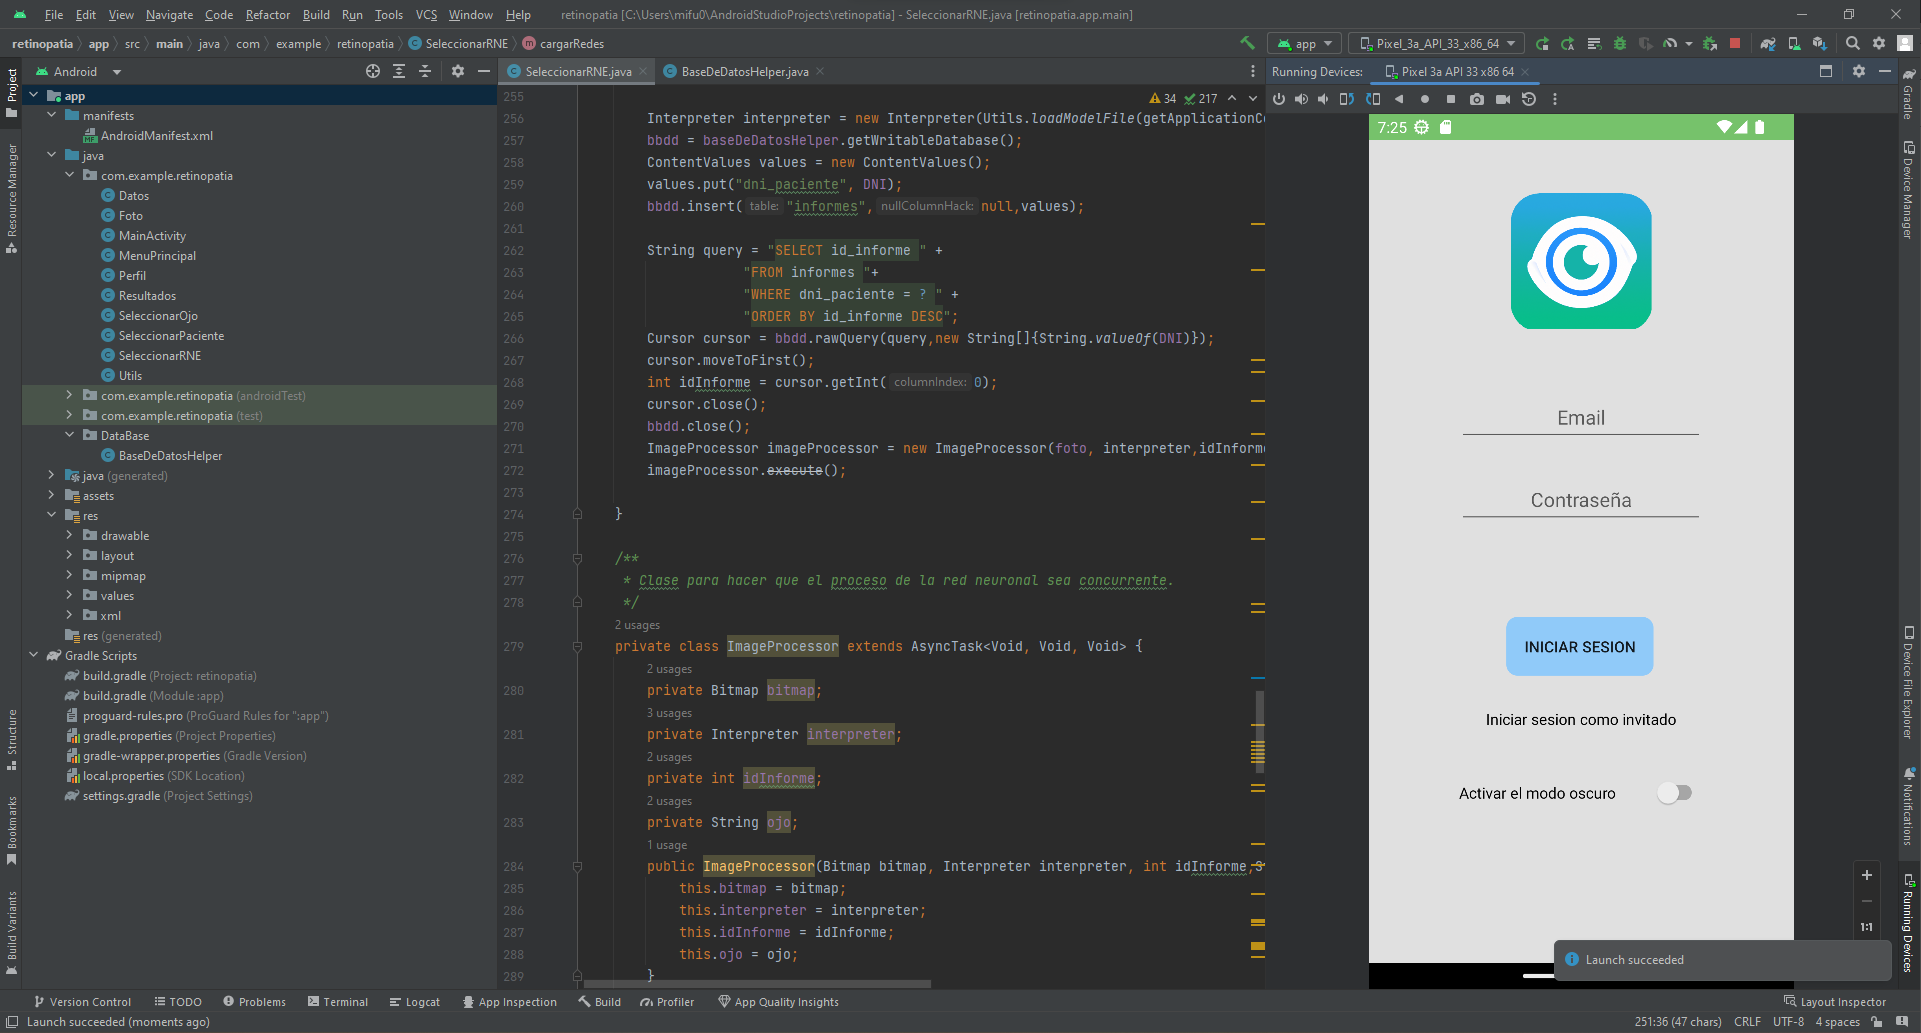
\includegraphics[width=0.9\textwidth]{img/Android Studio.png}
         \caption{Android Studio con un dispositivo virtual.}
         \label{fig:Android Studio}
\end{figure}
\begin{figure}[!ht]
         \centering
         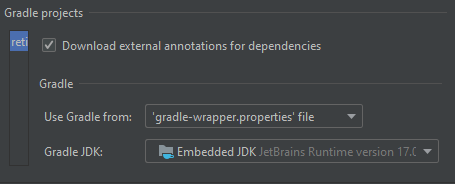
\includegraphics[width=0.9\textwidth]{img/JDK Graddle.png}
         \caption{Gradle incluye el JDK.}
         \label{fig:JDK}
\end{figure}
\begin{figure}[!ht]
         \centering
         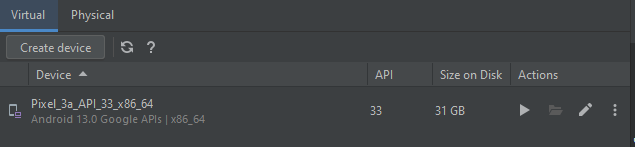
\includegraphics[width=0.9\textwidth]{img/AVD.png}
         \caption{Dispositivos virtuales Android.}
         \label{fig:AVD}
\end{figure}

\begin{figure}[!ht]
         \centering
         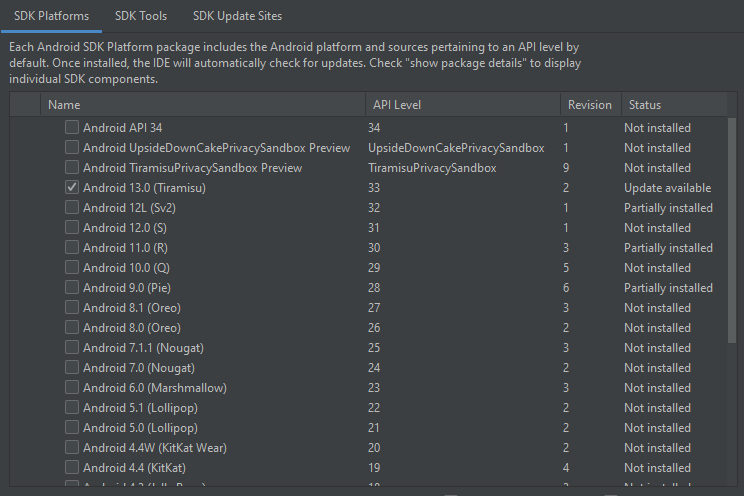
\includegraphics[width=0.9\textwidth]{img/SDK Android.png}
         \caption{SDKs ofrecidos.}
         \label{fig:SDK}
\end{figure}

\section{Compilación, instalación y ejecución del proyecto}

\subsection{Instalación}


Para instalar Android Studio, desde la página oficial se obtiene el ejecutable, puesto que es posible que el proyecto no sea compatible con futuras versiones de Android Studio, se ha utilizado la versión ``Flamingo 2022.2.1'', en caso de incompatibilidad, la página ofrece un aparatado para descargar \href{https://developer.android.com/studio/archive?hl=es-419}{versiones anteriores}.

Al descargar el ejecutable, se siguen las instrucciones, y el instalador instala automáticamente el SDK de Android y el emulador. Y el JDK se incluye en el Gradle del proyecto.

Para instalar Python, se descarga desde la página oficial, en este caso como ya es una versión anterior, se va al apartado de versiones anteriores y se descarga la versión 3.10.8.

Una vez instalado, se comprueba que la variable de entorno está configurada correctamente, en caso de no estarlo, el ``Path'' por defecto en Windows es: \textit{C:\textbackslash Users\textbackslash \$username\$\textbackslash AppData\textbackslash Local\textbackslash Programs\textbackslash Python\textbackslash Python310\textbackslash }. 

Para instalar las librerías de Python, se insertar 1 a 1 las siguientes líneas:

\lstdefinestyle{DOS}
{
    backgroundcolor=\color{black},
    basicstyle=\scriptsize\color{white}\ttfamily
}
\lstset{
  style=DOS,
  keywordstyle=\color{blue},
  commentstyle=\color{green!60!black},
  stringstyle=\color{red},
  showstringspaces=false,
  breaklines=true,
  breakatwhitespace=false,
  tabsize=4,
  numbers=none,
  numberstyle=\tiny,
  frame=single,
  framexleftmargin=5mm,
  xleftmargin=5mm
}
\begin{lstlisting}
cd C:\Users\$username$\AppData\Local\Programs\Python\Python310\Scripts\
pip install numpy
pip install pandas
pip install matplotlib
pip install scikit-learn
pip install tensorflow

\end{lstlisting}

Con las librerías instaladas, se procede a instalar el IDE, aunque también se puede usar un editor de texto y utilizar la consola para su ejecución. Como no es relevante el IDE que se utilice, no se comentará su instalación.

\subsection{Obtención del proyecto}

Para descargase el proyecto, se recomienda hacer uso de git. Para ello, se prepara el directorio donde se va a realizar el  proyecto, y posteriormente, se introduce el comando ``git clone https://github.com/mfg1014/Retinopatia-diabetica.git''.

Con el proyecto descargado, se pueden importar los archivos Python de la carpeta ``CNN y converter'' en el IDE que se use, en abrir carpeta. 

Para importar el proyecto Android, sería File > Open, y se selecciona la carpeta /app/retinopatía. Con ello, Android Studio detectará que es un proyecto Android, abriendo el proyecto para trabajar en él.

\subsection{Ejecución del proyecto}

Para el proyecto Python, la aplicación se ejecuta con el comando Python ``nombre del archivo''.py. Es importante tener en cuenta que el archivo de las redes neuronales tarda bastante, debido a que tiene que crear cada ejecución el modelo VGG-16, además, se crean 30 modelos, con sus respectivas matrices de confusión.

Para el proyecto Android se puede comprobar su ejecución de distintas formas:

\textbf{Emulador}

Android Studio ofrece un emulador incluido, donde se pueden probar las funcionalidades de la aplicación.

Para usar un emulador, se abre el Device manager, añadiendo un nuevo dispositivo, donde se selecciona entre varios dispositivos, en la realización de la práctica, se ha utilizado el dispositivo Pixel 3a con la versión Tiramisu, también se pueden seleccionar características como los núcleos de la CPU, la memoria RAM, el espacio del dispositivo,... Una vez creado, se abre el menú ``Run'', y se selecciona ``Run app''.

\textbf{Dispositivo físico}

Para usar un dispositivo físico es necesario habilitar las opciones de desarrollador, una vez hecho, se tiene que habilitar la opción de depuración ya sea por WIFI o por USB. Cuando se vincula con Android Studio, el dispositivo informa que se quiere añadir una aplicación mediante depuración, y una vez instalada se puede  usar como una aplicación normal.
\subsection{Errores encontrados y nuevas funcionalidades}

En caso de encontrar errores en la aplicación, se recomienda añadir una Issue al repositorio, donde se trabajará para solucionar el problema.

Si se quiere añadir nuevas funcionalidades, se recomienda crear una nueva rama por cada funcionalidad que se esté implementando concurrentemente.

\subsection{Crear una nueva realease}

Para crear una nueva release, es necesario obtener la apk para ello, en Android Studio, se hace lo siguiente:
\begin{itemize}
    \item Build > Build Bundle(s) /APK(s) > BUild APK(s).
    \item De esta forma, se genera el archivo .apk en el directorio ``app/build/outputs/apk/debug/''
\end{itemize}

Posteriormente, con el archivo APK, se comprime el directorio de la aplicación en un .zip y se va al repositorio al apartado releases, y se añade una nueva con estos archivos.

\section{Pruebas del sistema}

Como ya se ha comentado en el Diseño de pruebas, no se han realizado pruebas automáticas, pero cada vez que se realizaba un cambio de la aplicación, se comprobaba los casos de prueba relativos a las pruebas. Es importante aclarar que algunas funcionalidades no tienen pruebas específicas, pero de forma aleatoria se introducían en otros casos de prueba para comprobar el correcto funcionamiento.

Por otro lado, se han hecho pruebas en el emulador con una API Android 33 y en el dispositivo físico con una API Android 31. Por tanto, puede a ver errores en la visualización de los datos para versiones inferiores.

Mientras que en los archivos Python no es necesario el uso de pruebas.

Al finalizar el proyecto, todos los casos de prueba se pasaban correctamente.

\apendice{Documentación de usuario}

\section{Introducción}

\section{Requisitos de usuarios}

\section{Instalación}

\section{Manual del usuario}





\bibliographystyle{plain}


\end{document}
